\documentclass[letterpaper,12pt]{article}
\usepackage[top = 1in, bottom = 1in, left = 0.5in, right = 1in]{geometry}
\usepackage{inputenc}
\usepackage{graphicx}
\usepackage{amsmath}
\usepackage{amsfonts}
\usepackage{caption}
\usepackage{color}
\usepackage{listings}
\usepackage[framed,numbered,autolinebreaks,useliterate]{mcode}
%opening
\author{Gowtham Garimella}

\makeatletter
\newcommand\ackname{Acknowledgements}
\if@titlepage
  \newenvironment{acknowledgements}{%
      \titlepage
      \null\vfil
      \@beginparpenalty\@lowpenalty
      \begin{center}%
        \bfseries \ackname
        \@endparpenalty\@M
      \end{center}}%
     {\par\vfil\null\endtitlepage}
\else
  \newenvironment{acknowledgements}{%
      \if@twocolumn
        \section*{\abstractname}%
      \else
        \small
        \begin{center}%
          {\bfseries \ackname\vspace{-.5em}\vspace{\z@}}%
        \end{center}%
        \quotation
      \fi}
      {\if@twocolumn\else\endquotation\fi}
\fi
\makeatother

\newcommand{\executeiffilenewer}[3]{%
\ifnum\pdfstrcmp{\pdffilemoddate{#1}}%
{\pdffilemoddate{#2}}>0%
{\immediate\write18{#3}}\fi%
}
\newcommand{\includesvg}[1]{%
\executeiffilenewer{#1.svg}{#1.pdf}%
{inkscape -z -D --file=#1.svg %
--export-pdf=#1.pdf --export-latex}%
\input{#1.pdf_tex}%
}

\title{EN.530.603 Applied Optimal Control \\HW \#2 Solutions}
\graphicspath{{./figures/}}
\begin{document}
\maketitle

\begin{enumerate}

  %%%%%%%%%%%%%%%Question 1%%%%%%%%%%%%%%%%%%%%%%%%
  \item To find the curve $x^*$ which minimizes J(x) passing throught 0 and 4.
  \begin{equation}
   J(x) = \int_0^1 \left[ \frac{1}{2} {\dot x}^2(t) + 3 x(t) \dot x(t) +2x^2(t) + 3x(t)\right]dt
  \end{equation}
  From Euler-Lagrange equations:
  \begin{align*}
   &&J(x) = \int_0^1 g(x,\dot x,t) dt \\
    &\text{Necessary Conditions}& \\
  &&g_x - \frac{d}{dt} g_{\dot x}  = (3 \dot x + 4x + 3) - \frac{d}{dt}(\dot x + 3x) = 0\\
   &&\Rightarrow \ddot x = 4x + 3 \\ 
   &\text{Homogenous solution:}&\\
   &&\ddot x = 4x \Rightarrow x(t) = \lambda_1 e^{2t} + \lambda_2 e^{-2t} \quad \lambda_1 , \lambda_2 \in \mathbf{R} \\
   &\text{Non Homogenous solution:}&\\
   &&x(t) = -3/4 \Rightarrow \ddot x = 0 = 4 ( -3/4) +3\\
   &\text{Combined Solution:}&\\
   && x(t) =  \lambda_1 e^{2t} + \lambda_2 e^{-2t} - \frac{3}{4} \\
   &\text{Boundary Conditions:}& \\
   &&x(1) = 4 \quad \& \quad x(0) = 0\\
   &&\Rightarrow \lambda_1 + \lambda_2 = 3/4\\
   &&\Rightarrow \lambda_1 e^2 + \lambda_2 e^{-2} = 19/4\\
   && \Rightarrow \lambda_1 = \frac{-3 e^{-2} + 19}{4(e^2 - e^{-2})} = 0.6408\quad \lambda_2 = \frac{3 e^{2} - 19}{4(e^2 - e^{-2})} = 0.1091 \\ 
  \end{align*}
  Thus the final solution for extremal trajectory x(t) is given as:
  \begin{equation*}
   x(t) = 0.6408e^{2t} + 0.1091 e^{-2t} - 0.75
  \end{equation*}

  %%%%%%%%%%%%%%%Question 2%%%%%%%%%%%%%%%%%%%%%%%%
  \item To find extremals for 
  \begin{align*}
    J(x) &= \int_0^{t_f} [{\dot{x_1}}^2(t) + {\dot{x_2}}^2(t) + 3 x_1(t) x_2(t) ] dt\\
    g(x,\dot{x}) &= [{\dot{x_1}}^2(t) + {\dot{x_2}}^2(t) + 3 x_1(t) x_2(t) ]
  \end{align*}
  Using necessary conditions on the trajectory, the Euler-Lagrange equations give the extremal trajectory as:
  \begin{align*}
  g_x - \frac{d}{dt} g_{\dot x}  &= \left[ 3 x_2 \quad 3 x_1\right] - \frac{d}{dt} \left[ 2 \dot{x_1}\quad 2\dot{x_2}\right] = 0\\
  \Rightarrow 2 \ddot{x_1} &= 3 x_2 \quad \& \quad 2 \ddot{x_2} = 3 x_1 \\
  \Rightarrow x_1^{(4)} &= \frac{3}{2} \ddot{x_2} = \frac{9}{4} x_1 \\
  \Rightarrow x_1(t) &= \lambda_1 sinh(\omega t) + \lambda_2 sin(\omega t) + \lambda_3 cosh(\omega t) + \lambda_4 cos(\omega t) \quad \omega = \sqrt{3/2};\\
  \Rightarrow x_2(t) &= \frac{2}{3} \ddot{x_1} = \lambda_1 sinh(\omega t) - \lambda_2 sin(\omega t) + \lambda_3 sinh(\omega t) - \lambda_4 sin(\omega t) \enskip \lambda_{1,2,3,4} \in \mathbb{R}\\
  \end{align*}
  Given $x_1(0) = 0 \enskip x_2(0) = 0$ implies that:
  \begin{equation*}
   \lambda_3 + \lambda_4 = 0 \enskip \& \enskip \lambda_3 - \lambda_4 = 0
  \end{equation*}
  which gives $\lambda_3 = \lambda_4 = 0$.
  
  \begin{align}
  \Rightarrow x_1(t) &= \lambda_1 sinh(\omega t) + \lambda_2 sin(\omega t) \label{eqn:2.axt}\\
  \Rightarrow x_2(t) &= \frac{2}{3} \ddot{x_1} = \lambda_1 sinh(\omega t) - \lambda_2 sin(\omega t) \label{eqn:2.bxt} 
  \end{align}

  \begin{enumerate}
   \item Given the boundary conditions we evaluate the unknowns $\lambda_1$ and $\lambda_2$ :
   \begin{align*}
    &\text{If} \enskip t_f = 1 \text{ and } x_2(t_f) = 1 \\
    &\text{then} \enskip \lambda_1 sinh(\omega) - \lambda_2 sin(\omega) = 1 \quad \text{ From Eqn[\ref{eqn:2.axt}]}\\
    &\text{If} \enskip x_1(t_f) \text{ is free } \\
    &\text{then} \enskip g_{\dot x} (1) |_{t_f} = \begin{bmatrix}
                                                   2 \dot{x_1}(t_f) & 2 \dot{x_2}(t_f)\\
                                                  \end{bmatrix}(1)
 = 0 \\
    &\Rightarrow \enskip 2 \dot{x_1}(t) |_{t = 1} = 0\\
    &\Rightarrow \enskip \lambda_1 cosh(\omega) + \lambda_2 cos(\omega) = 0\\
    &\Rightarrow \enskip
			  \begin{bmatrix}
			    sinh(\omega) & -sin(\omega)\\
			    cosh(\omega) & cos(\omega) \\
			  \end{bmatrix} 
			  \begin{bmatrix}
                          \lambda_1 \\
			  \lambda_2 \\
                         \end{bmatrix} = 
			 \begin{bmatrix}
			  1 \\
			  0\\
			 \end{bmatrix}\\
    &\Rightarrow 	  \begin{bmatrix}
                          \lambda_1 \\
			  \lambda_2 \\
			 \end{bmatrix} = \frac{1}{\alpha} 
			 \begin{bmatrix}
			  cos(\omega)\\
			  -cosh(\omega)\\
			 \end{bmatrix}\\
			 &\text{where} \enskip \alpha = cos(\omega) sinh(\omega) +cosh(\omega) sin(\omega) \\
   \end{align*}
   This solves the optimization problem for the given boundary conditions completely as 
   \begin{align*}
    x_1(t) &= \frac{1}{\alpha} (cos(\omega) sinh(\omega t) -cosh(\omega) sin(\omega t))\\
    x_2(t) &= \frac{1}{\alpha} (cos(\omega) sinh(\omega t) + cosh(\omega) sin(\omega t))\\
    \omega &= \sqrt{3/2} \enskip \& \enskip \alpha = cos(\omega) sinh(\omega) +cosh(\omega) sin(\omega) \\
   \end{align*}
   
   \item Given $t_f$ is free but the final position should lie on the surface:
   \begin{equation*}
   \psi(x(t),t) = x_1(t) + 3 x_2(t) + 5 t - 15 = 0
   \end{equation*}
   With this boundary condition, the optimization problem is modified as 
   \begin{align*}
    J^{\prime} (x) &= \nu (\psi(x(t_f), t_f)) + \int_0^{t_f} g(x,\dot x, t) dt\\
    g(x,\dot x, t) &= {\dot{x_1}}^2(t) + {\dot{x_2}}^2(t) + 3 x_1(t) x_2(t) 
   \end{align*}
   which provides the necessary boundary conditions as:
   \begin{align*}
   g_{\dot x} (t_f) + \nu (\psi_x(t_f)) &= 0 \\
   g(t_f) - g_{\dot x}(t_f) \dot x(t_f) + \nu (\psi_t(t_f)) &= 0 \\
   \psi(x(t_f),t_f) &= 0\\
   \end{align*}
   We need to solve for the unknowns $t_f, \lambda_1, \lambda_2, \nu$ with the conditions as described below.
   \begin{align*}
   g_{\dot x} (t_f) + \nu (\psi_x(t_f)) &= 0 \\
   \Rightarrow 2 \begin{bmatrix}
               \dot x_{1}(t_f) & \dot x_{2}(t_f)
               \end{bmatrix} + \nu 
	       \begin{bmatrix}
	        1 & 3 
	       \end{bmatrix} &= 0 \\
    \Rightarrow \dot{x}(t_f) = \frac{-\nu}{2} \theta \enskip \text{where } \theta &= [1 \enskip 3]^{T}\\
    \Rightarrow \dot x(t_f) = \omega \begin{bmatrix}
                cosh(\omega t_f) & cos(\omega t_f) \\
		cosh(\omega t_f) & - cos(\omega t_f) \\
                \end{bmatrix} 
		\begin{bmatrix}
		 \lambda_1\\
		 \lambda_2 \\
		\end{bmatrix} &= -\frac{\nu}{2} 
		\begin{bmatrix}
		 1 \\
		3 
		\end{bmatrix} \quad \text{From Eqns(\ref{eqn:2.axt}, \ref{eqn:2.bxt})}\\
	\Rightarrow 
		\begin{bmatrix}
		 \lambda_1\\
		 \lambda_2 \\
		 \end{bmatrix} &= \frac{\nu}{2 \omega}
		 \begin{bmatrix}
		  -2 sech(\omega t_f)\\
		  sec(\omega t_f) \\
		 \end{bmatrix}\\
	\Rightarrow x(t_f) = 
			  \begin{bmatrix}
			    sinh(\omega t_f) & sin(\omega t_f)\\
			    sinh(\omega t_f) & -sin(\omega t_f) \\
			  \end{bmatrix} 
			  \begin{bmatrix}
                          \lambda_1 \\
			  \lambda_2 \\
                         \end{bmatrix} &=  \frac{\nu}{2 \omega}
			 \begin{bmatrix}
			  -2tanh(\omega t_f) + tan(\omega t_f)\\
			  -2tanh(\omega t_f) - tan(\omega t_f)\\
			 \end{bmatrix}
    \end{align*}
    Now using the above conditions, we solve for $\nu$ in terms of $t_f$ using the second boundary condition:
   %\Rightarrow g(t_f) = \dot{x}(t_f)^{T} \dot{x}(t_f)+ 3 x_{1f} x_{2f}  =\frac{\nu}{4}\theta^{T} \theta + 3 x_{1f} x_{2f}  &= \frac{5}{2}\nu^2 + 3 x_{1f} x_{2f}\\
    \begin{align*}
   g(t_f) - g_{\dot x}(t_f) \dot x(t_f) + \nu (\psi_x(t_f)) &= 0 \\
   \Rightarrow \dot{x}(t_f)^{T} \dot{x}(t_f)+ 3 x_{1}(t_f) x_{2}(t_f) - 2 \dot{x}(t_f)^{T} \dot{x}(t_f) + 5\nu &= 0\\
   \Rightarrow -\frac{5}{2}\nu^2 + 3 x_{1f} x_{2f} + 5\nu &= 0\\
   \Rightarrow -\frac{5}{2}\nu^2 + 5\nu + \frac{ \nu^2}{2} (4 tanh^2(\omega t_f) - tan^2(\omega t_f)) &= 0\\
   \nu \left[ 4 tanh^2(\omega t_f) - tan^2(\omega t_f) -5 \right] &= -10\quad \text{Since } \nu \neq 0 \\
   \end{align*}
   Now we use the third condition which requires the final point to be on the surface to find the final time $t_f$ which solves all the other variables in terms of $t_f$:
   \begin{align*}
    \theta^{T} x(t_f) + 5t_f - 15 &= 0\\
    \Rightarrow \frac{\nu}{2 \omega} \theta^{T} 
    \begin{bmatrix}
    -2tanh(\omega t_f) + tan(\omega t_f)\\
    -2tanh(\omega t_f) - tan(\omega t_f)\\
  \end{bmatrix} + 5t_f - 15 &= 0\\ 
  \Rightarrow \frac{\nu}{2 \omega} (-8 tanh(\omega t_f) -2 tan(\omega t_f) ) + 5t_f - 15 &= 0\\
\end{align*}
The above equation is solved in MATLAB to obtain the value of $t_f$. The function has multiple solutions \{3.6665, 4.3404, 5.9142, 7.2788, 8.1885\}. The family of extremals is given by:
\begin{align*}
 t_f &= \{3.6665, 4.3404, 5.9142, 7.2788, 8.1885\}\\
 \omega &= \sqrt{3/2}\\
 \nu &= \frac{-10}{4 tanh^2(\omega t_f) - tan^2(\omega t_f) -5 }\\
 \begin{bmatrix}
  \lambda_1 \\
  \lambda_2 \\
 \end{bmatrix} &= \frac{\nu}{2 \omega}
  \begin{bmatrix}
    -2 sech(\omega t_f)\\
    sec(\omega t_f) \\
  \end{bmatrix}\\
 x_1(t) &= \lambda_1 sinh(\omega t) + \lambda_2 sin(\omega t) \\
 x_2(t) &= \lambda_1 sinh(\omega t) - \lambda_2 sin(\omega t) \\
\end{align*}
We pick $t_f = 3.6665$ to verify the constraints. The initial boundary conditions are obvious since $sinh(0) = sin(0) = 0:\enskip x_1(0) = x_2(0) = 0$. For the final time, we have to ensure the 
trajectory lies on the surface $\psi(x(t_f),t_f) = 0$
\begin{align*}
x_1(t_f = 3.665) &= -0.0089 sinh(3.665\omega) -0.8982 sin(3.665\omega) = 0.4810\\
x_2(t_f = 3.665) &= -0.0089 sinh(3.665\omega) +0.8982 sin(3.665\omega) =-1.2714 \\
\psi(x(t_f),t_f) &= [1\enskip 3] \begin{bmatrix}
                           0.4810 \\
                           -1.2714
                          \end{bmatrix} + 5(3.6488) - 15 = -3.333 -15 + 18.325 = 0.00082 \sim 0 
\end{align*}
Similar checks can be done for other solutions also.
  \end{enumerate}
  \newpage
  %%%%%%%%%%%%Question 3%%%%%%%%%%%%%%%%%%%%%
  \item Given a function $\eta(t) \in \mathbf{C}^2$ (twice continous) defined on $\{t_0, t_f\}$ such that $\eta(t_0) = \eta(t_f) = 0$. We need to derive the Euler-Lagrange necessary conditions for fixed boundary conditions using the following evaluation form:
  \begin{align*}
   &J(x) = \int_{t_0}^{t_f} g(x(t), \dot x(t), t) dt \\
   &\left.\frac{d J(x^* + \epsilon \eta) }{d \epsilon} \right|_{\epsilon = 0} = 0 \\[5pt]
   &\Rightarrow \int_{t_0}^{t_f} \left.\frac{d g(x^* + \epsilon \eta, {\dot x}^* + \epsilon \dot \eta)}{d \epsilon}\right|_{\epsilon = 0} dt = 0\\
   &\Rightarrow \frac{dg(x^* + \epsilon \eta,{\dot x}^* + \epsilon \dot \eta)}{d \epsilon} = \frac{\partial g}{\partial (x^* + \epsilon \eta)} \frac{d(x^* + \epsilon \eta)}{d\epsilon} + \frac{\partial g}{\partial (\dot x^* + \epsilon \dot \eta)} \frac{d(\dot x + \epsilon \dot \eta)}{d\epsilon}\\
   &\Rightarrow  \left. \frac{dg(x^* + \epsilon \eta,{\dot x}^* + \epsilon \dot \eta)}{d \epsilon}\right|_{\epsilon = 0} = \frac{\partial g}{\partial x^* } \eta + \frac{\partial g}{\partial \dot x^*} \dot \eta\\
   &\Rightarrow \int_{t_0}^{t_f} \left( \frac{\partial g}{\partial x^*} \eta  + \frac{\partial g}{\partial \dot x^*} \dot \eta \right) dt = 0\\
   &\Rightarrow \int_{t_0}^{t_f} \frac{\partial g}{\partial x^*} \eta(t) dt +\left. \frac{\partial g}{\partial \dot x^*} \eta(t)\right|_{t_0}^{t_f} - \int_{t_0}^{t_f} \frac{d}{dt} \left( \frac{\partial g}{\partial \dot x^*} \right) \eta (t) dt = 0 \\
   &\Rightarrow \int_{t_0}^{t_f} \left[ \frac{\partial g}{\partial x^*} - \frac{d}{dt} \left( \frac{\partial g}{\partial \dot x^*} \right)\right] \eta (t) dt = 0 \quad \text{Since } \eta(t_0) = \eta (t_f) = 0\\
  \end{align*}
  Since $\eta(t)$ is arbitrary function except for the endpoints, the above function will be zero only if the pre-multiplier to $\eta$ is zero over the trajectory between $t_0 $ and $t_f$. This gives the Euler-Lagrange equations as:
  \begin{equation*}
  \Rightarrow  \frac{\partial g}{\partial x} - \frac{d}{dt} \left( \frac{\partial g}{\partial \dot x} \right) = 0 \quad \forall x(t) = x^*(t) \enskip t \in \{t_0,t_f\} 
  \end{equation*}
  %%%%%%%%%%%%%%%%Question 4%%%%%%%%%%%%%%%%%
  \item Given optimization problem :
  \begin{align*}
   \dot x &= ax - bu \quad x(t_0) \text{ given}\\
   J  &= \frac{1}{2} c \left[ x(t_f) \right]^2 + \frac{1}{2} \int_{t_0}^{t_f} \left[ u(t) \right]^2 dt
  \end{align*}
  Equating the relevant parts of this problem to the general optimization problem we get the following:
  \begin{align*}
   &J_a = \phi(x(t_f),t_f) + \int_{t_0}^{t_f}\left( H(x(t),u(t),\lambda, t), -\lambda^T \dot x\right) dt \quad \text{(General optimization problem)}\\
   &\phi(x(t_f),t_f) =  \frac{1}{2} c \left[ x(t_f) \right]^2 \\
   &H(x(t),u(t),\lambda, t) = \frac{1}{2} \left[ u(t) \right]^2 + \lambda(ax - bu) \\
  \end{align*}
  The necessary conditions for optimal control is :
  \begin{align*}
   H_u &= u - \lambda b = 0 \\
   \Rightarrow u &= \lambda b\\
   \dot \lambda &= - \partial_x H = -a \lambda \\
   \Rightarrow \lambda &= m e^{-at}\\
   \Rightarrow u &= m b e^{-at}\\
  \end{align*}
  With this input we solve the dynamics of the system as follows:
  \begin{align*}
   \dot x &= ax - b(m b e^{-at}) \\
   \Rightarrow x(t) &= e^{a(t-t_0)} x(t_0) + \int_{t_0}^{t} e^{a(t-\tau)} b \left( -m e^{-a \tau } b \right) d\tau\\
   \Rightarrow x(t) &= e^{a(t-t_0)} x(t_0) - \frac{m b^2 e^{at}}{2a} \left[ -e^{-2at} + e^{-2at_0}\right]\\
  \end{align*}
  Now we apply the boundary condition for $\lambda$ to get the value of m :
  \begin{align*}
   \lambda(t_f) &= \left. \partial_x \phi(x,t) \right|_{t=t_f} \\
   \Rightarrow \lambda(t_f) &= c x(t_f) = c \left[e^{a(t_f-t_0)} x(t_0) - \frac{m b^2 e^{at_f}}{2a} \left( e^{-2at_0} - e^{-2at_f}\right) \right]\\
   \Rightarrow m e^{-at_f} &= c e^{a(t_f - t_0)} x(t_0) - m \{ \frac{cb^2 e^{at_f}}{2a} \left(e^{-2at_0} - e^{-2at_f}\right)\}\\
   \Rightarrow m &= \frac{c e^{a(t_f - t_0)} x(t_0)} { e^{-at_f} + \frac{cb^2 e^{at_f}}{2a}\left( e^{-2at_0} - e^{-2at_f}\right)}\\
  \end{align*}
  Which solves the problem by providing explicitly the control u(t) as:
  \begin{equation*}
  u(t) = mbe^{-at} = \frac{bc e^{a(t_f - t_0)} x(t_0)} { 1 + \frac{cb^2}{2a}\left( e^{2a(t_f-t_0)}-1\right)}e^{a(t_f-t)}
  \end{equation*}
  This can be show after a lot of intermediate steps to be equivalent to:
  \begin{equation*}
   u(t) = \frac{bc e^{2a(t_f - t)}}{1 - \frac{b^2 c}{2a} \left( 1 - e^{2a(t_f - t)}\right)}x(t)
  \end{equation*}
  (Note: This problem can also be easily solved using riccati equation and arrive at the second solution. The steps for the second method are outlined as below:)
  The Riccati equation for the above problem is given as:
  \begin{equation*}
   \dot P = -2aP + P^2 b^2
  \end{equation*}
  Substituting $b^2 P = \frac{-\dot q}{q}$, we get:
  \begin{equation*}
   \ddot q + 2a \dot q = 0
  \end{equation*}
  Using boundary conditions $q(t_f) = 1, \dot q(t_f) = -c b^2$, we get :
  \begin{align*}
   q(t) &= \left(1 - \frac{cb^2}{2a}\right)  + \frac{c b^2}{2a} e^{2a(t_f - t)}\\
   P(t) &=  \frac{c e^{2a(t_f - t)}}{1 - \frac{cb^2}{2a}\left(1 - e^{2a(t_f - t)}\right)}
  \end{align*}
  Then the control can be specified as:
  \begin{equation*}
   u(t) = bP(t) x(t) = \frac{bc e^{2a(t_f - t)}}{1 - \frac{b^2c}{2a}\left(1 - e^{2a(t_f - t)}\right)} x(t)
  \end{equation*}
  The solution matches with the above solution and shows the linear feedback form for the control in LQR type of problems.





 %%%%%%%%%%%%%%%%%%%%%%%%%Question 5%%%%%%%%%%%%%%%%%%%%%%%%%
 \item The matlab code for the problem is given below:
  \lstinputlisting[language=Matlab]{hw2.m}
  The results of the above code are shown below:
  \begin{figure}[h!]
   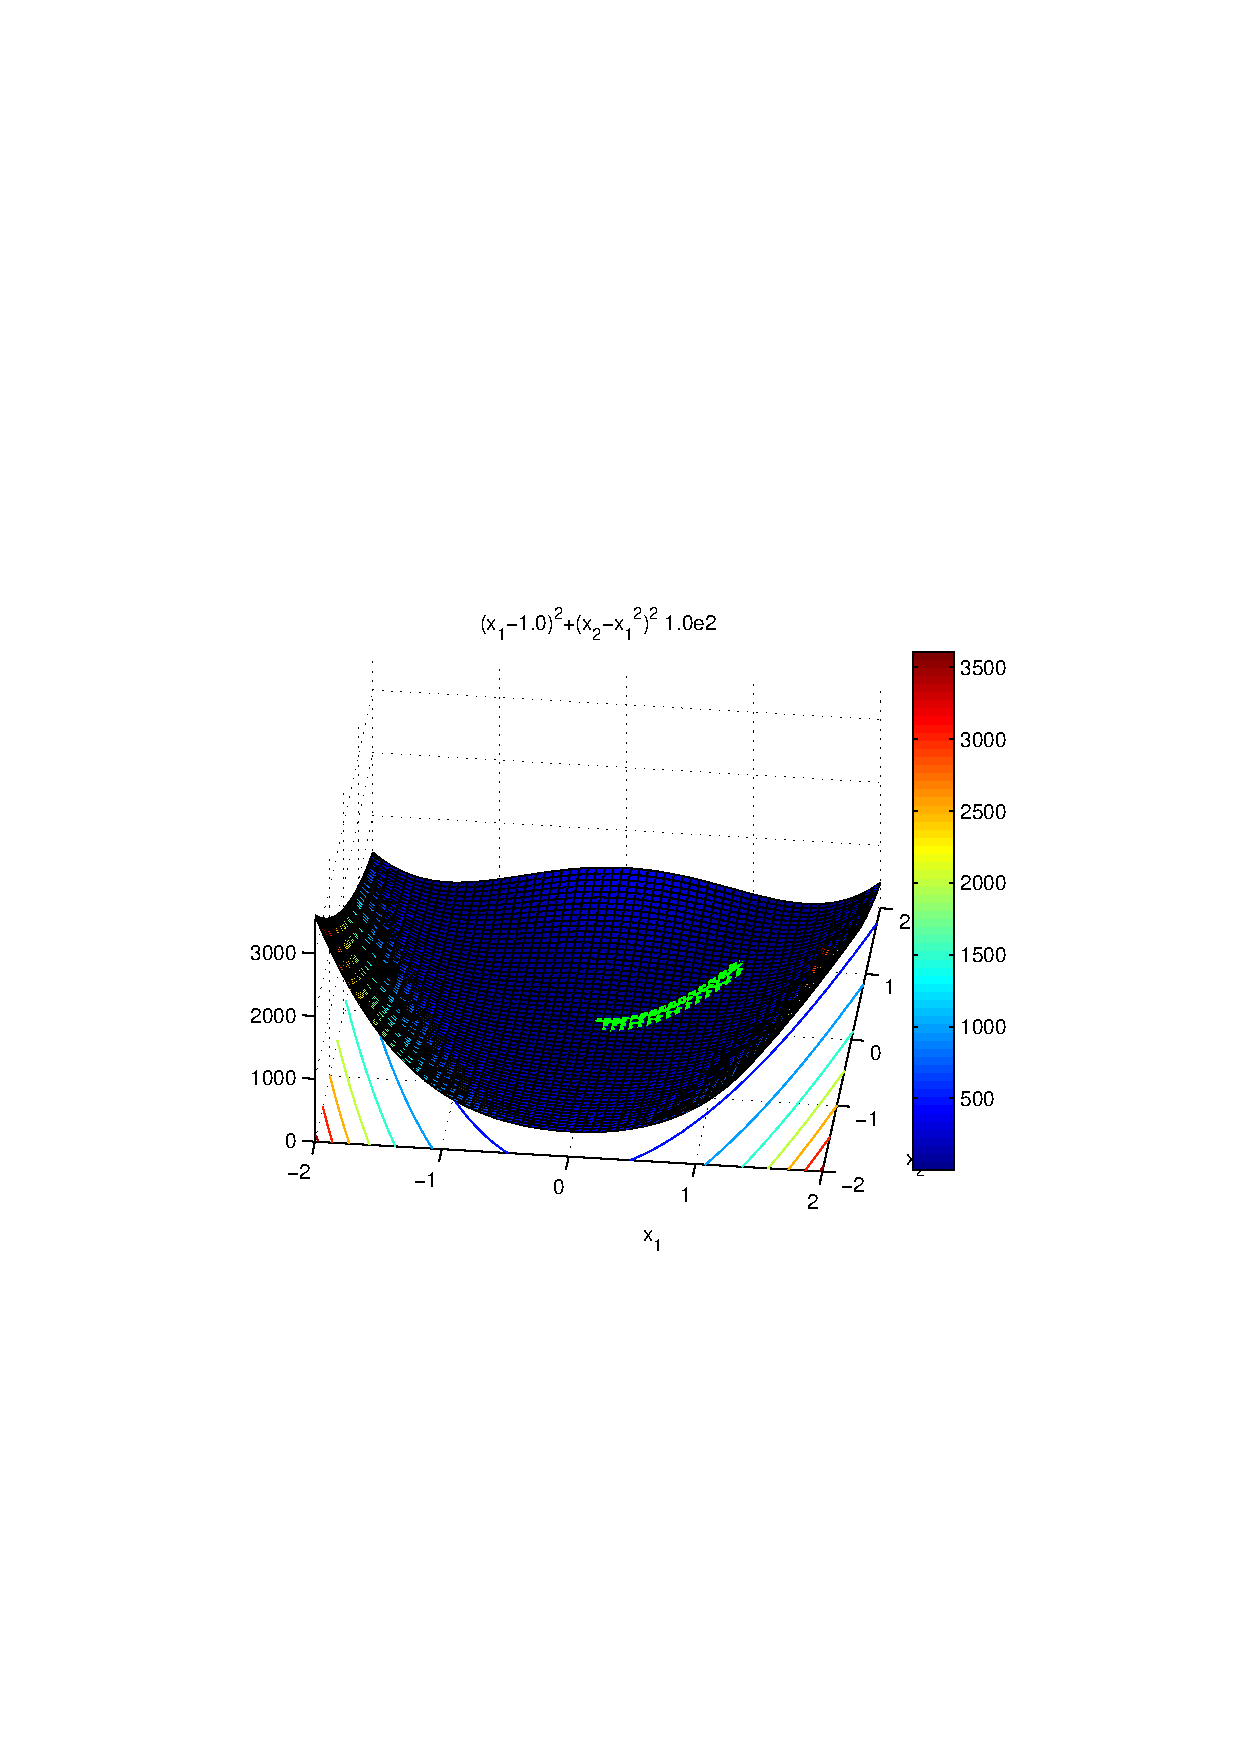
\includegraphics[width=\linewidth]{pic1.pdf}
   \caption{The solution to riccati equation P(t) with Pf = 0}
   \label{fig1}
  \end{figure}
  \begin{figure}[h!]
   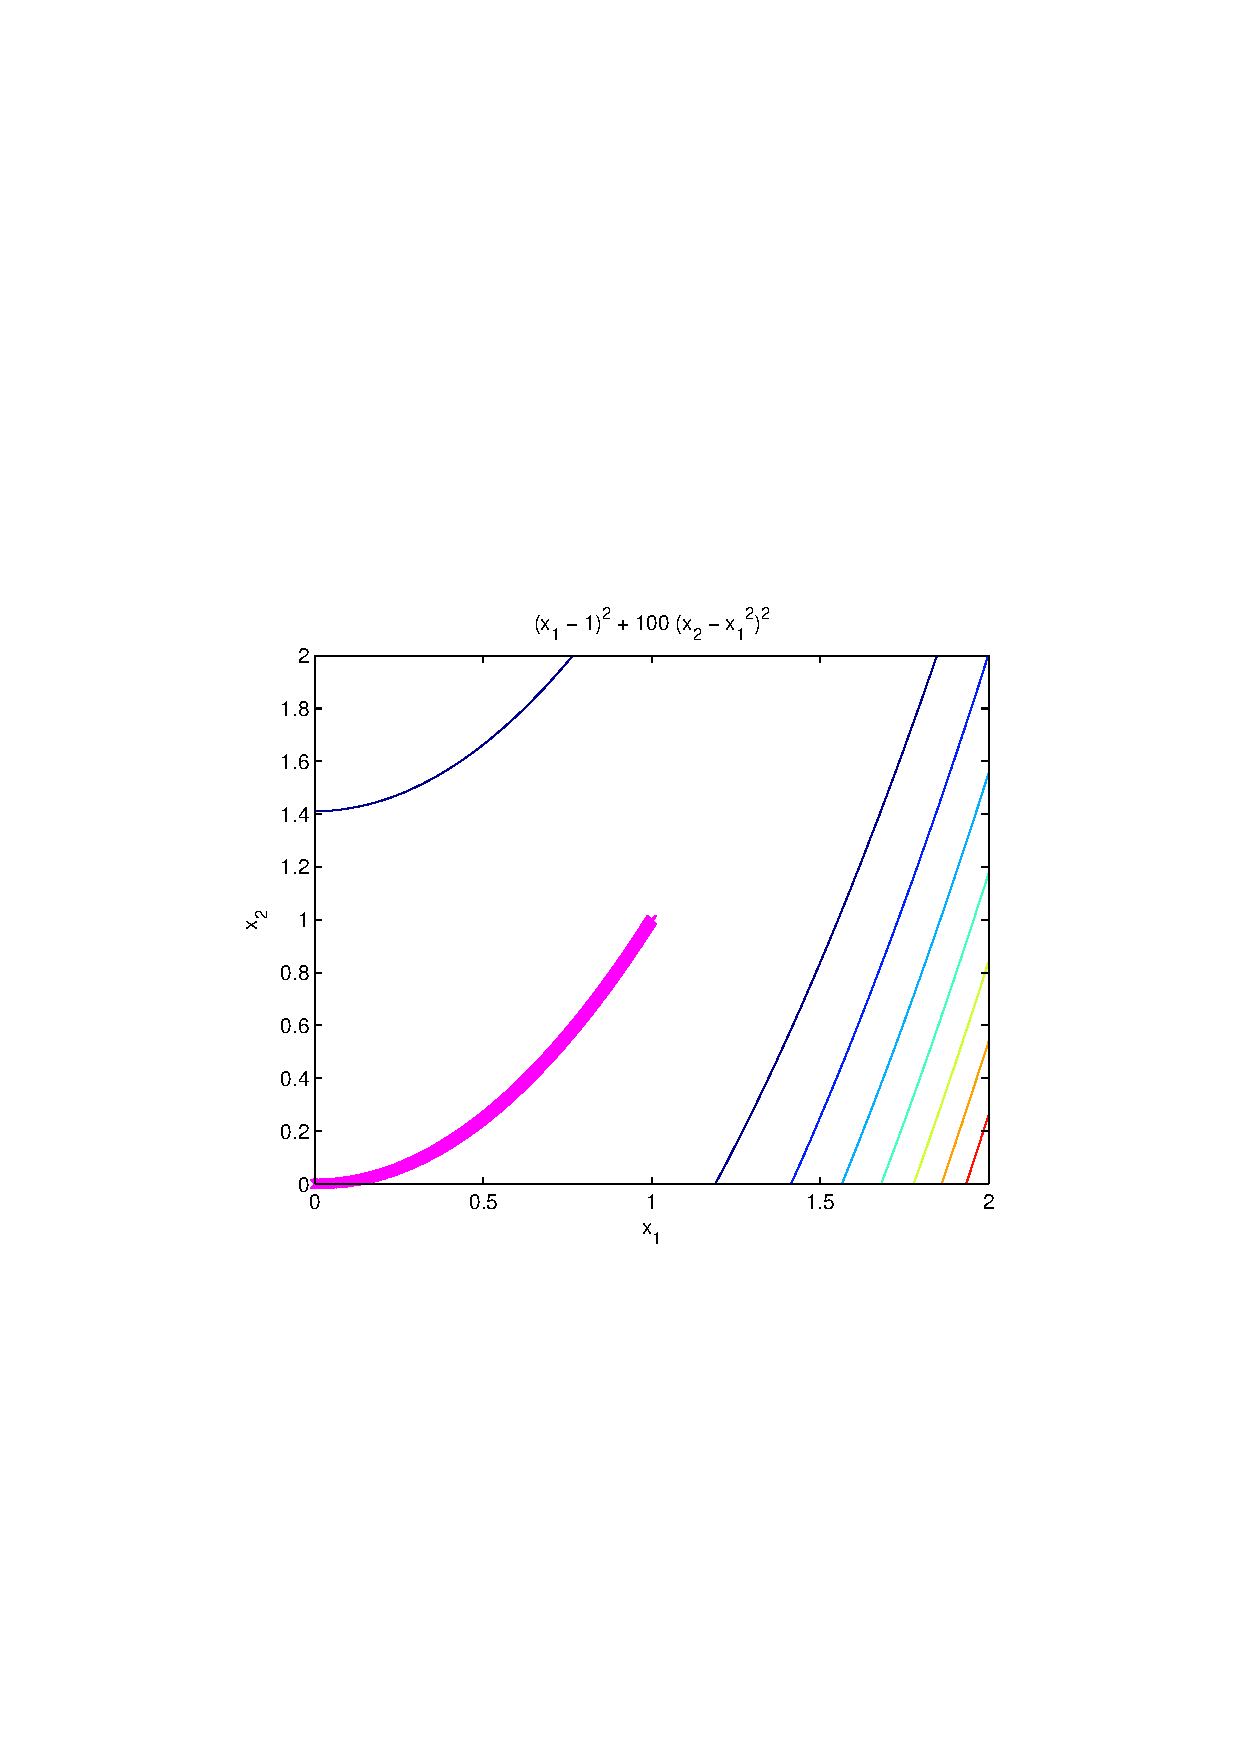
\includegraphics[width=\linewidth]{pic2.pdf}
   \caption{The state X(t) and the control U(t)}
  \end{figure}
  \newpage
  
  
  %%%%%%%%%%%%%%%%Question 6%%%%%%%%%%%%%%%%%
  \item Riccati equations are 	first order differential equations with a special structure i.e equations have maximum differential order 1 and maximum polynomial order of the 
  variable as 2. Riccati equations can be written in the form[Source \textbf{Wiki}]:
  \begin{equation*}
   y^{\prime}(x) = q_0(x) + q_1(x) y(x) + q_2(x) y^2 (x)
  \end{equation*}
  This equation can be reduced to second order linear differential equation [Source \textbf{Wiki}]:
  \begin{align*}
   &\text{Substituting: } y(x) q_2(x) = \frac{-u^{\prime}}{u}\\
   &\Rightarrow y(x) {q_2}^\prime(x) + y^\prime(x)q_2(x) = \frac{-u^{\prime\prime}}{u} + \left(\frac{u^{\prime}}{u}\right)^2\\
   &\Rightarrow y(x) {q_2}^\prime(x) + \{q_0(x) + q_1(x) y(x) + q_2(x) y^2(x)\} q_2(x) = \frac{-u^{\prime\prime}}{u} + \left(\frac{u^{\prime}}{u}\right)^2\\
   &\Rightarrow q_2(x) q_0(x) +  y(x) \{{q_2}^\prime(x)+ q_2(x) q_1(x)\} + q_2(x)^2 y^2(x)  = \frac{-u^{\prime\prime}}{u} + \{q_2(x) y(x)\}^2 \\
   &\Rightarrow u^{\prime\prime} = -q_2(x) q_0(x) u - uy(q_2 q_1 + {q_2}^\prime) \\
   & \text{Using}: R(x) = q_1(x) + \frac{q_2^\prime (x)}{q_2(x)} \quad S(x) = q_2(x) q_0(x) \quad u^\prime = -u(x)y(x)q_2(x)\\
   & u^{\prime\prime} -R u^{\prime} + S u = 0
  \end{align*}
  The second order equation can be solved to compute the solutions for y(x)\\
  
  \centering{\textbf{[THIS is just for your information; I don't expect everyone to write this]}}
%   About Riccati:\\ 
%   Riccati is an Italian Mathematician born in 1676. He was self educated in Mathematics by reading then current day's mathematical journals.  His major contributions were in solving differential equations. He is best known for Riccati equation named 
%   after him.[Source Wiki, http://www-history.mcs.st-and.ac.uk/Mathematicians/Riccati.html]

\end{enumerate} 
\vfill
\begin{acknowledgements}
I hereby declare that I have not discussed this homework with anyone. The solutions written here are my own work and  from lecture notes and sample code provided by the professor. Any 
external references are mentioned in the text.
\flushright Gowtham Garimella
\end{acknowledgements}




\end{document}
